% 中文版，用 xelatex 编译：xelatex research_note_zh && xelatex research_note_zh
\documentclass[11pt,UTF8]{ctexart}
\usepackage[margin=1in]{geometry}
\usepackage{amsmath,amssymb,booktabs,graphicx,float,xcolor}
\usepackage[round,authoryear]{natbib}
\usepackage[hidelinks]{hyperref}

\newcommand{\E}{\mathbb{E}}
\newcommand{\1}{\mathbf{1}}
\renewcommand{\arraystretch}{1.12}
\setlength{\abovecaptionskip}{4pt}
\setlength{\belowcaptionskip}{6pt}
\renewcommand{\refname}{参考文献}

\title{尾部风险模型能否提供波动率与相关性之外的信息？\\
\large 来自多资产市场的证据}
\author{Shangrong Li\thanks{研究笔记，未经同行评审。代码与取数 notebook：
\url{https://github.com/lshangro-png/tail-risk-cn}。全部结果均可由免费公开数据重新生成。本文译自英文版。}}
\date{2026 年 10 月}

\begin{document}
\maketitle

\begin{abstract}
\noindent
尾部风险方法（copula 尾部相关、预期损失（ES）预算）在卖方研究中被广泛推介，被视为对基于波动率和相关系数的风险管理的改进。
本文研究的问题是：这些方法是否携带了波动率和相关系数所没有的信息。我们在中国及全球大类资产上做了两项检验。
\emph{检验一}将尾部相关统计量与高斯 copula 零假设比较，后者在每个估计区间内都与观测到的相关系数矩阵相匹配。
实践中使用的单参数 Clayton/Gumbel 系数与该零假设在统计上无法区分：它们与普通相关系数的秩相关在数据中为 0.94，
在零假设下也是 0.94。带独立尾部参数的模型在六资产周度面板中确实检测到了相关性之外的尾部相关
（105 个 Student-$t$ 对高斯检验中有 31 个在 5\% 水平下拒绝，匹配零假设下的期望为 5.7 个），
且集中在风险资产之间和下尾；而在中国股票与国债之间，证据较弱，也没有下行不对称。
\emph{检验二}把尾部风险平价拆成两个组成部分：用 ES 代替波动率，以及以 GARCH 波动率预测作条件。
用 ES 代替波动率使超额夏普比率提高 0.00--0.04，均不显著。条件化在扣除成本前带来约 0.11 的提升，
但把年化单边换手从 15\% 提高到 95\%，在每单位交易 25 个基点的成本下这一提升完全消失。
预备部分表明，按 250 个观测校准的 Acerbi--Szekely $Z_2$ 阈值 $-0.70$ 在长样本回测中不提供信息，
并以一个带 wild bootstrap $p$ 值的自归一化检验替代。在本文研究的市场和样本内，
这些尾部风险方法相对于跟踪当前波动率和相关性的增量价值很小。
\end{abstract}

% ---------------------------------------------------------------------------
\section{引言}

波动率和线性相关系数只描述多元收益分布的二阶矩。尾部风险方法承诺更多：copula 尾部相关系数意在刻画相关系数遗漏的联合暴跌
\citep{embrechts2002}，预期损失（ES）则是对超过在险价值（VaR）部分损失的一致性度量。国内卖方研报已将这些思想变成交易规则，
例如由滚动 Clayton 与 Gumbel 尾部系数触发的股债``双杀''预警、基于下尾距离的层次配置，以及尾部风险平价 \citep{alankar2013}。
本文要回答的问题很窄：\emph{在已知当前波动率和相关性的条件下，这些尾部风险统计量是否增加了信息？}

有两个难点使这个问题比看上去更难。第一，自然的基准并不是独立。对正相关数据拟合单参数阿基米德 copula，
即使真实 copula 是没有尾部相关的高斯 copula，也会得到正的尾部系数。因此零假设必须固定相关系数。
第二，基于 ES 的配置与基于波动率的配置之所以不同，可能有两个独立的原因：风险度量变了，而用于估计它的情景又常常以当前波动率为条件。
这两种效应必须分开，并且比较时要扣除各自产生的换手成本。

本文有三点贡献。(i)~对一组尾部相关统计量构造\emph{相关系数匹配}的高斯 copula 零假设，
同时处理相关性混淆以及共享同一资产的检验之间的相关性。(ii)~把尾部风险平价拆成 $2\times 2$ 设计（风险度量 $\times$ 条件化），
并在两种明确的执行规则下，结合实际换手与交易成本进行评估。(iii)~表明常用于 ES 回测的固定 $Z_2$ 阈值在长样本中未经校准，
并给出一个简单的替代方法。

对卖方研报的完整复现及代码见配套仓库。本文概括其中最有力的两条证据。

% ---------------------------------------------------------------------------
\section{数据}

全部数据来自免费公开来源：中债官网（债券财富指数）、通过 AkShare 获取的新浪、腾讯和东方财富数据（中国指数与 ETF）、
FRED（汇率、布伦特原油、波动率指数）以及 Kenneth French 数据库。价格存放在本地 SQLite 数据库中，所有结果都由它重新计算。

\begin{itemize}
\item \textbf{单资产回测（第~\ref{sec:marginal}~节）。}上证 50、沪深 300、中证 500 指数，中债综合财富指数，
黄金（GLD $\times$ 美元兑人民币），标普 500 和布伦特原油的日收益，起始于 1987--2006 年（视序列而定），截至 2026 年 10 月。
\item \textbf{股债对（第~\ref{sec:test1}~节）。}沪深 300 与中债综合财富指数，日度，2003--2026 年。两者在北京时间同时收盘。
\item \textbf{多资产面板（第~\ref{sec:test1}~节）与配置（第~\ref{sec:test2}~节）。}
沪深 300、中证 500、标普 500、中债国债总财富指数（CGB）、人民币计价黄金和布伦特原油。
中国与西方市场收盘时间不同，会使同日相关偏向零，因此相关性检验使用\emph{周}收益（周五至周五）。
配置回测为月度调仓，使用 2005 年至 2026 年 10 月的日收益（5{,}008 个共同交易日）。
\item \textbf{ETF 面板。}十只境内上市 ETF（国内股票风格、纳斯达克、恒生、黄金、商品），2016--2026 年，用于下尾距离的比较。
\end{itemize}

% ---------------------------------------------------------------------------
\section{预备：边际尾部与校准的 ES 回测}
\label{sec:marginal}

在检验相关性之前，先看对单个资产而言什么是重要的。我们在滚动 1{,}000 日窗口上运行六种一日 VaR/ES 预测方法：
历史模拟、正态、Student-$t$、GPD 超阈值（POT）、带过滤历史模拟（FHS）的 GJR-GARCH(1,1)，
以及在标准化残差上拟合 GPD 尾部的 GJR-GARCH \citep[GARCH-EVT；][]{mcneil2000,glosten1993}。
99\% VaR 用 \citet{kupiec1995} 无条件覆盖检验和 \citet{christoffersen1998} 独立性检验评估，
97.5\% ES 用 \citet{acerbi2014} 的 $Z_2$ 统计量评估。

\paragraph{$Z_2$ 检验需要零分布，而不是固定阈值。}
设 $X_t$ 为收益，$\mathrm{VaR}_t$ 与 $\mathrm{ES}_t$ 为水平 $\alpha$ 下的预测（均取正数），$I_t = \1\{X_t < -\mathrm{VaR}_t\}$。
Acerbi 和 Szekely 定义
\begin{equation}
Z_2 = \frac{1}{T\alpha}\sum_{t=1}^{T}\frac{X_t I_t}{\mathrm{ES}_t} + 1 .
\end{equation}
记 $Y_t = X_t I_t/\mathrm{ES}_t + \alpha$，则 $Z_2 = \sum_t Y_t/(T\alpha)$。若两个预测都正确，
$\E_{t-1}[X_t I_t] = -\alpha\,\mathrm{ES}_t$，从而 $\E_{t-1}[Y_t]=0$：无论波动率如何变化，$\{Y_t\}$ 都是鞅差序列。
Acerbi 和 Szekely 给出的 5\% 近似临界值 $-0.70$ 是在 $T=250$ 下模拟得到的。$Z_2$ 在零假设下的标准差按 $1/\sqrt{T\alpha}$ 缩小，
因此在 $T\approx 5{,}000$ 日的回测中，固定的 $-0.70$ 对应小得多的检验水平和低得多的功效。为此我们使用自归一化统计量
\begin{equation}
S = \frac{\sum_t Y_t}{\sqrt{\sum_t Y_t^2}} \xrightarrow{d} N(0,1)\quad\text{（在 } H_0 \text{ 下）},
\end{equation}
这由鞅中心极限定理得到 \citep{hallheyde1980}。有限样本 $p$ 值用 wild bootstrap 计算：
$S^{*} = \sum_t Y_t\varepsilon_t/\sqrt{\sum_t Y_t^2}$，其中 $\varepsilon_t$ 为独立的 Rademacher 变量 \citep{wu1986,mammen1993}。
检验是单侧的：显著为负的 $S$ 意味着 ES 偏小或 VaR 突破过于频繁。相关的累积突破方法见 \citet{duescanciano2017}。

\paragraph{蒙特卡洛检验。}
表~\ref{tab:z2mc} 模拟一个标准化 $t_5$ 新息的 GARCH(1,1)（$\omega=0.02$，$\alpha=0.08$，$\beta=0.90$，收益以百分比计），
并评估 97.5\% ES 的三种预测：真实的条件 VaR 与 ES；使用真实波动率的正态尾部，它把 ES 低估 14\%，而 VaR 只低估 1.6\%；
以及把真实预测乘以 0.85。当 $T=250$ 时，规则 $Z_2<-0.70$ 在 5.3\% 的样本中拒绝正确模型，与设计一致。
当 $T=5{,}000$ 时，它从不拒绝正确模型，从未识别出正态尾部，对 15\% 的缩放也只在 37\% 的样本中识别出来。
基于 $S$ 的检验在 $T=5{,}000$ 时水平为 4.3\%，对两种设定错误的功效分别为 62\% 和 100\%。
在 $T=250$ 时渐近检验偏保守（水平 1.7\%；一年只有约六次 97.5\% 突破），应使用 wild bootstrap $p$ 值。
在下文的长样本回测中，渐近 $p$ 值与 bootstrap $p$ 值之差不超过 0.03。

\begin{table}[t]
\centering
\caption{GARCH(1,1)（标准化 $t_5$ 新息）1{,}000 次模拟中 97.5\% ES 回测的拒绝率。“规则”：$Z_2<-0.70$。“检验”：基于 $S$ 的 5\% 单侧渐近检验。}
\label{tab:z2mc}
\small
\begin{tabular}{lrrrr}
\toprule
 & \multicolumn{2}{c}{$T=250$} & \multicolumn{2}{c}{$T=5000$} \\ \cmidrule(lr){2-3}\cmidrule(lr){4-5}
预测 & 规则 & 检验 & 规则 & 检验 \\
\midrule
正确模型 & 5.3\% & 1.7\% & 0.0\% & 4.3\% \\
正态尾部、波动率正确 & 15.7\% & 4.5\% & 0.0\% & 61.5\% \\
VaR 与 ES 均乘以 0.85 & 44.5\% & 25.3\% & 37.0\% & 100.0\% \\
\bottomrule
\end{tabular}
\end{table}


\paragraph{结果。}
表~\ref{tab:var} 给出每种方法下、七个资产中各项检验在 5\% 水平下不拒绝的资产个数。在固定阈值下，
正态模型对七个资产中的六个``通过''了 ES 回测，尽管其实际尾部损失比预测 ES 高出 27\%（中位数）。
在校准检验下，它对全部七个资产都被拒绝。不更新波动率的方法（历史模拟、Student-$t$、GPD）的无条件覆盖大致正确，
但突破会聚集：在一次突破的次日再次突破的概率为 4--15\%，而不是 1\%，Christoffersen 检验对七个资产中的六个拒绝。
它们的 ES 对三到五个资产被拒绝。两种 GARCH 过滤方法几乎对每个资产都通过了全部三项检验；
在过滤残差上加 GPD 尾部（GARCH-EVT）比 FHS 略微改善了聚集性（6/7 对 5/7）。

\begin{table}[t]
\centering
\caption{七个资产的一日 VaR/ES 回测（滚动 1{,}000 日窗口）。第 3--6 列为 7 个资产中该检验在 5\% 水平下不拒绝的个数。“旧规则”：$Z_2>-0.70$。“校准检验”：自归一化统计量 $S$ 的单侧 wild bootstrap $p$ 值。最后一列：在 97.5\% VaR 突破日上，平均实际损失与平均预测 ES 之比，取各资产的中位数。}
\label{tab:var}
\small
\resizebox{\linewidth}{!}{\begin{tabular}{lrrrrrr}
\toprule
方法 & 99\% VaR 突破率 & Kupiec & Christoffersen & $Z_2$ 旧规则 & $Z_2$ 校准检验 & 损失/ES \\
\midrule
历史模拟 & 1.22\% & 5/7 & 1/7 & 7/7 & 4/7 & 1.03 \\
正态 & 1.83\% & 0/7 & 0/7 & 6/7 & 0/7 & 1.27 \\
Student-$t$ & 1.13\% & 3/7 & 1/7 & 7/7 & 2/7 & 1.00 \\
GPD（POT） & 1.12\% & 5/7 & 1/7 & 7/7 & 4/7 & 1.03 \\
GARCH-FHS & 1.07\% & 7/7 & 5/7 & 7/7 & 7/7 & 1.03 \\
GARCH-EVT & 0.97\% & 7/7 & 6/7 & 7/7 & 7/7 & 1.03 \\
\bottomrule
\end{tabular}}
\end{table}


对后文的启示是：在单资产层面，真正重要的信息是当前波动率。在 GARCH 过滤之上再做尾部形状建模（EVT 对 FHS）改变不大。

% ---------------------------------------------------------------------------
\section{检验一：相关性之外的尾部相关}
\label{sec:test1}

\subsection{为什么单参数尾部系数主要度量的是相关性}

Clayton copula $C_\theta(u,v) = (u^{-\theta}+v^{-\theta}-1)^{-1/\theta}$ 的下尾相关为 $\lambda_L = 2^{-1/\theta}$；
Gumbel copula 的上尾相关为 $\lambda_U = 2-2^{1/\theta}$。每个族只有一个参数，同时决定正相关的整体强度和尾部。
当真实 copula 是相关系数 $\rho>0$ 的高斯 copula 时，用任一族去拟合，极大似然会让 $\theta$ 离开独立边界以匹配整体相关，
于是尽管真实尾部相关为零，$\hat\lambda$ 仍为正 \citep{joe1997}。因此合适的零假设是相关系数相同的高斯 copula，而不是独立。

在沪深 300--中债综合这一对上，按中金（2021）预警规则使用滚动 60 日窗口时，这一点影响很大。
在 $\rho=0.3$ 的高斯 copula 中，按点估计规则已有 94\% 的 60 日窗口给出 $\hat\lambda_L>0$。
仅用 60 日相关系数就能以 0.95 的 AUC 区分 $\hat\lambda_L>0$ 与 $\hat\lambda_L=0$ 的交易日。
与匹配每个窗口正态得分相关系数的高斯零假设相比，观测到的 $\hat\lambda_L>0$ 频率为 33.4\%，期望为 34.5\%；
中金触发条件（$\hat\lambda_L>0$ 且 $\hat\lambda_U=0$）的频率为 4.8\%，期望为 4.7\%。这个信号就是时变相关性本身所能产生的。
在十只 ETF 的面板中，两两 Clayton $\hat\lambda_L$（250 日窗口）与普通相关系数的秩相关在各调仓日平均为 0.98；
用 $\hat\lambda_L$ 的组合 ES 加总公式并不比用 $\rho$ 的更准确（绝对误差中位数 2.2\% 对 2.0\%）。

\subsection{带独立尾部参数的模型}

要回答是否存在\emph{超出}相关性的尾部相关，模型需要一个与整体相关参数分开的尾部参数。我们使用两种模型。

\emph{Student-$t$ 对高斯 copula。}$t$ copula 有相关系数 $\rho$ 和自由度 $\nu$；
其尾部相关
\[
\lambda = 2\,t_{\nu+1}\!\left(-\sqrt{(\nu+1)(1-\rho)/(1+\rho)}\right)
\]
在 $\nu\to\infty$ 时趋于零，此时退化为高斯 copula \citep{demarta2005}。
在相同的 $\rho$ 下，有限的 $\nu$ 意味着极端值比高斯 copula 所隐含的更常同时出现。
$H_0:\nu=\infty$ 的似然比统计量位于参数空间边界上，因此其零分布为 $\tfrac12\chi^2_0+\tfrac12\chi^2_1$，$p=\tfrac12 P(\chi^2_1\ge \mathrm{LR})$。

\emph{对称化 Joe--Clayton（SJC）copula} \citep{patton2006}。它的两个参数就是下尾和上尾相关系数 $\tau_L,\tau_U$，
因此 $H_0:\tau_L=\tau_U$ 是一个单约束的尾部不对称似然比检验。

对股债对，我们在每个自然年内做 $t$ 检验（窗口互不重叠，因此可以用二项检验统计拒绝次数）。
它在 23 年中有 4 年在 5\% 水平下拒绝高斯，期望为 1.15 年（二项 $p=0.026$）；用过去 60 日波动率标准化收益后，22 年中有 7 年拒绝（$p=10^{-4}$）。
隐含的尾部相关很小（滚动 250 日窗口上的中位数为 0.2\%）。方向是对称的：两者同日落入各自最差 10\% 的有 57 次，
同日落入最好 10\% 的有 55 次，高斯 copula 下的期望为 47.5 次。SJC 检验没有发现下行不对称
（在有可测尾部相关的五个年份上合并 $p=0.79$）。在中国股票与国债之间，相关性之外的尾部相关很弱，也不偏向联合暴跌。

\subsection{带相关系数匹配零假设的多资产面板}

股债只是一对资产。我们把检验扩展到六个配置资产的全部 15 对，周收益分为七个互不重叠的三年区间
（2005--2025 年，每段 139--153 周），共得到 105 个资产对--区间。在每个区间内，把秩转换为伪观测值，
并对每一对记录 $t$ 对高斯的 $p$ 值、$t$ 隐含的 $\lambda$、SJC 估计值及其不对称 $p$ 值、Clayton $\hat\lambda_L$，
以及两个资产同时落入各自最低（最高）十分位的周数。

\paragraph{零假设。}共享同一资产的检验彼此相关，因此拒绝次数不服从二项分布；而且对强相关的资产对，$t$ 检验略有水平扭曲
（$\rho=0.6$、156 个观测时为 8\%）。这两个问题都通过在零假设下模拟整个面板来处理。在每个区间中，
零假设是一个六维高斯 copula，其相关矩阵等于该区间的正态得分相关矩阵。因此它复现了截面相关结构及其在区间之间的变化，
且没有尾部相关。我们模拟同样长度的数据，完全按观测数据的方式重新计算每个统计量，重复 200 次。
每个汇总统计量都与其模拟零分布比较，单侧 $p$ 值为 $(1+\#\{s^*\ge s\})/(1+200)$。

\begin{table}[t]
\centering
\caption{多资产面板（6 个资产、15 对，周收益分为 7 个互不重叠的三年区间，共 105 个资产对--区间）与相关系数匹配的高斯 copula 零假设（200 次模拟）的比较。$p$：模拟得到的单侧 $p$ 值（统计量偏大方向）。波动率标准化：收益除以过去 26 周的波动率。}
\label{tab:panel}
\small
\resizebox{\linewidth}{!}{\begin{tabular}{lrrrrrr}
\toprule
 & \multicolumn{3}{c}{原始周收益} & \multicolumn{3}{c}{波动率标准化} \\ \cmidrule(lr){2-4}\cmidrule(lr){5-7}
统计量 & 观测值 & 零假设均值 [5\%, 95\%] & $p$ & 观测值 & 零假设均值 & $p$ \\
\midrule
$t$ 对高斯拒绝数（5\%） & 31 & 6 [1, 10] & 0.005 & 31 & 6 & 0.005 \\
平均 $t$ 隐含 $\lambda$ & 0.063 & 0.018 [0.010, 0.028] & 0.005 & 0.064 & 0.018 & 0.005 \\
下尾 10\% 同落周数 & 302 & 235 [212, 257] & 0.005 & 299 & 226 & 0.005 \\
上尾 10\% 同落周数 & 251 & 231 [207, 257] & 0.104 & 226 & 224 & 0.438 \\
下尾 $-$ 上尾 & 51 & 4 [-25, 32] & 0.015 & 73 & 3 & 0.005 \\
SJC 平均 $\hat\tau_L-\hat\tau_U$ & 0.049 & 0.000 [-0.016, 0.018] & 0.005 & 0.055 & 0.001 & 0.005 \\
SJC 不对称拒绝数（5\%） & 8 & 2 [0, 5] & 0.005 & 7 & 2 & 0.010 \\
平均 Clayton $\hat\lambda_L$ & 0.096 & 0.082 [0.073, 0.093] & 0.015 & 0.094 & 0.079 & 0.020 \\
Spearman($\hat\lambda_L,\rho$) & 0.94 & 0.94 [0.92, 0.96] & 0.512 & 0.94 & 0.94 & 0.413 \\
\bottomrule
\end{tabular}}
\end{table}


\begin{figure}[t]
\centering
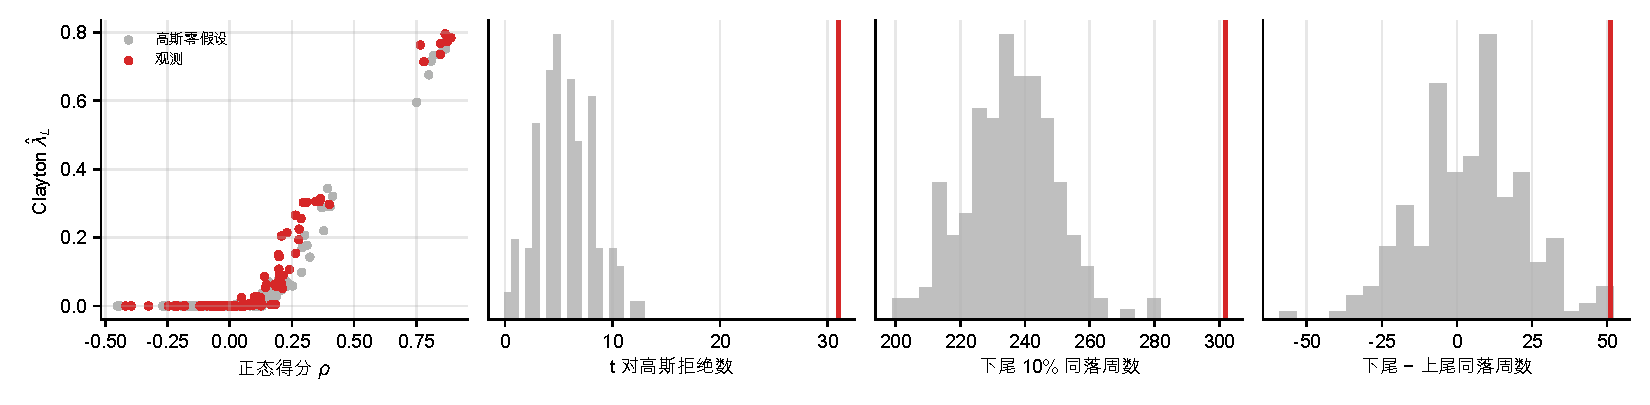
\includegraphics[width=\textwidth]{figures/zh/fig_panel.pdf}
\caption{多资产面板，原始周收益。左：105 个资产对--区间（红）以及匹配高斯零假设的一次模拟（灰）中，
Clayton $\hat\lambda_L$ 与正态得分相关系数的关系。其余各图：三个汇总统计量的零分布（灰）与观测值（红线）。}
\label{fig:panel}
\end{figure}

表~\ref{tab:panel} 和图~\ref{fig:panel} 给出了两个明确的回答。

\emph{Clayton 系数不携带相关性之外的信息。}它与 $\rho$ 的秩相关在数据中为 0.94，在零假设下也是 0.94；
平均 $\hat\lambda_L$ 只比零假设下略高（0.096 对 0.082）。无论尾部相关是否存在，卖方规则所用的这个统计量几乎完全是相关系数的单调函数。

\emph{相关性之外的尾部相关确实存在，且在下尾更强。}$t$ 检验在 105 个资产对--区间中拒绝 31 个，匹配零假设下期望为 5.7 个（$p<0.01$）。
同落下尾十分位的周数比同落上尾十分位的周数多 51，零假设下为 4（$p=0.015$），SJC 估计平均而言 $\tau_L>\tau_U$。
用过去 26 周波动率标准化收益（去除共同的波动率状态）后，这些结果不变或略有增强。$t$ 检验的拒绝分布在许多资产对上，
包括部分涉及国债的资产对。但下尾的超额来自风险资产之间：标普 500--布伦特（同落下尾 29 周，上尾 18 周）、
黄金--布伦特（26 对 13）和沪深 300--标普 500（26 对 16）。涉及国债的资产对没有下尾超额。

因此检验一的答案取决于统计量。相关性之外的尾部相关在周度数据中可以被统计检测到，且风险资产之间存在下尾超额。
但实践中使用的单参数系数看不到它；而在中国股票与债券之间，也就是大多数股债预警规则针对的那一对，它很小且对称。

% ---------------------------------------------------------------------------
\section{检验二：ES 风险预算是否增加价值？}
\label{sec:test2}

\subsection{设计}

风险平价选择仅做多的权重 $w$，使每个资产对风险度量 $R$ 的贡献相等。对正齐次的 $R$，等风险贡献组合为 $w=y^*/\mathbf{1}'y^*$，其中
\begin{equation}
y^* = \arg\min_{y>0}\; R(y) - \sum_{i=1}^{n} b_i\log y_i ,\qquad b_i = 1/n,
\end{equation}
只要 $R$ 是凸的，这就是一个凸问题 \citep{spinu2013,maillard2010}。对波动率，$R(y)=\tfrac12 y'\Sigma y$
（二次型，与 $\sqrt{y'\Sigma y}$ 得到相同的解）。对情景 $x_1,\dots,x_T$ 上水平 $q$ 的 ES，
\citet{rockafellar2000} 的表示在目标函数内部给出一个线性规划：
\begin{equation}
R(y) = \min_{a,\;u\ge 0}\; a + \frac{1}{(1-q)T}\sum_{t=1}^{T}u_t \quad\text{s.t.}\quad u_t\ge -x_t'y - a .
\end{equation}
即使对冲资产在等权下的贡献为负（不动点迭代在这种情况下会失败，\citealp{mausser2018}），这一形式在最优点也能保持所有 ES 贡献为正且相等。

四个策略构成 $2\times 2$ 设计：

\begin{center}
\begin{tabular}{lcc}
\toprule
 & 无条件情景 & 条件（FHS）情景 \\
\midrule
波动率预算 & RP & 条件 RP \\
ES 预算（$q=95\%$） & TRP（历史） & 条件 TRP \\
\bottomrule
\end{tabular}
\end{center}

无条件情景为最近 500 个日收益。条件情景是用每个资产各自的单变量 GJR-GARCH(1,1) 过滤同样的收益，
再缩放到明日预测波动率（多元 FHS，\citealp{baroneadesi1999}）。这保留了残差的历史截面相关结构，同时更新了尺度。
ES 效应是固定情景下的行差；条件化效应是列差。

\paragraph{执行与成本。}目标权重在每个月末计算，于下一交易日开盘生效。我们评估两种执行规则，二者都逐日跟踪实际持仓：
\emph{每日再平衡}回到目标（恒定比例策略），以及\emph{月度调仓、期间持有}，即两次调仓之间权重随价格漂移。
每个交易日的交易量为 $\sum_i|w_{i,t}^{\text{target}}-w_{i,t^-}|$，其中 $w_{t^-}$ 为漂移后的持仓，
并从当日收益中扣除每单位交易 $c\in\{0,10,25,50\}$ 个基点的成本。年化单边换手为年化交易量的一半。
超额夏普比率（无风险利率 2\%）之差用移动区块 bootstrap 评估（区块长度 20 日，重抽样 2{,}000 次；\citealp{kunsch1989}），
它保留了波动率聚集；同一问题的 HAC 推断方法见 \citet{ledoit2008}。

\subsection{结果}

\begin{table}[t]
\centering
\caption{尾部风险平价分解，2007 年 7 月至 2026 年 10 月，每月末用 500 日窗口计算目标权重。换手率为实际年化单边换手。超额夏普比率（无风险利率 2\%）按月度调仓、期间持有口径计算，已扣除列标题所示的单位交易成本。}
\label{tab:trp}
\footnotesize
\resizebox{\linewidth}{!}{\begin{tabular}{lrrrrrr}
\toprule
 & \multicolumn{2}{c}{换手率} & \multicolumn{4}{c}{超额夏普（单位交易成本）} \\ \cmidrule(lr){2-3}\cmidrule(lr){4-7}
策略 & 每日 & 月度 & 0 bp & 10 bp & 25 bp & 50 bp \\
\midrule
RP & 53\% & 15\% & 0.93 & 0.92 & 0.91 & 0.89 \\
TRP（历史） & 54\% & 16\% & 0.97 & 0.96 & 0.95 & 0.92 \\
条件 RP & 136\% & 95\% & 1.04 & 0.99 & 0.91 & 0.77 \\
条件 TRP & 134\% & 95\% & 1.06 & 1.00 & 0.92 & 0.77 \\
\midrule
\multicolumn{7}{l}{\emph{超额夏普之差（月度调仓、期间持有）：估计值 [95\% 区块 bootstrap 区间]}} \\
\multicolumn{3}{l}{ES 效应（条件情景）} & +0.02 [-0.06, +0.09] & +0.01 [-0.06, +0.09] & +0.01 [-0.06, +0.08] & 0.00 [-0.07, +0.07] \\
\multicolumn{3}{l}{ES 效应（无条件情景）} & +0.04 [-0.02, +0.11] & +0.04 [-0.03, +0.10] & +0.04 [-0.03, +0.10] & +0.03 [-0.03, +0.10] \\
\multicolumn{3}{l}{条件化效应（波动率）} & +0.11 [-0.07, +0.30] & +0.07 [-0.12, +0.25] & 0.00 [-0.18, +0.18] & -0.12 [-0.30, +0.07] \\
\multicolumn{3}{l}{条件 TRP $-$ RP} & +0.13 [-0.08, +0.33] & +0.08 [-0.13, +0.29] & +0.01 [-0.20, +0.21] & -0.12 [-0.32, +0.09] \\
\bottomrule
\end{tabular}}
\end{table}


\begin{figure}[t]
\centering
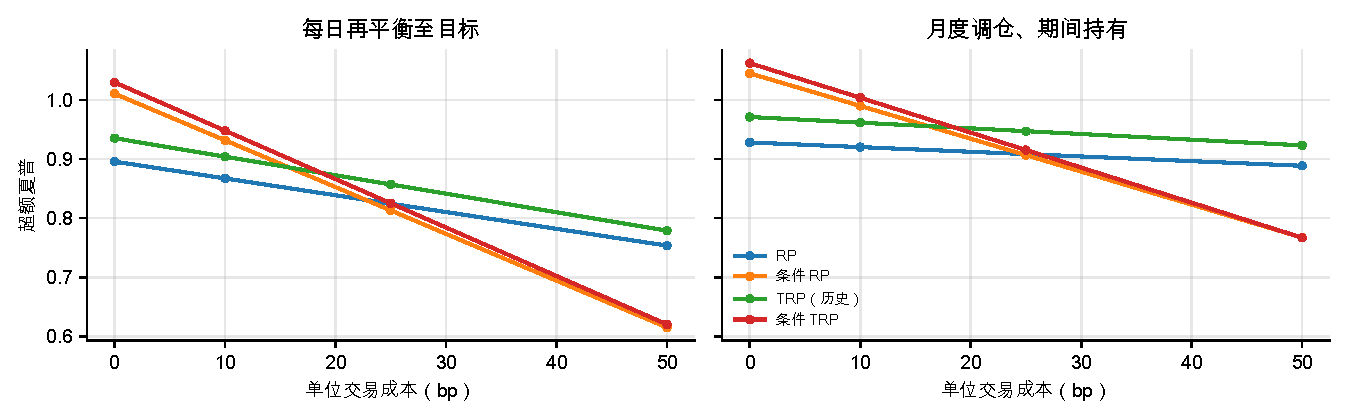
\includegraphics[width=0.92\textwidth]{figures/zh/fig_trp_costs.pdf}
\caption{超额夏普比率与单位交易成本的关系，2007-07 至 2026-10。}
\label{fig:costs}
\end{figure}

表~\ref{tab:trp} 和图~\ref{fig:costs} 总结了 2007 年 7 月至 2026 年 10 月的回测。

以下数字均指月度调仓、期间持有；每日再平衡得到相同的结论，只是换手更高。

\emph{用 ES 代替波动率几乎没有增益。}固定情景时，ES 预算在扣除成本前使超额夏普比率在无条件情景下提高 0.04，
在条件情景下提高 0.02。两者都不显著（bootstrap 95\% 区间为 $[-0.02,0.11]$ 和 $[-0.06,0.09]$）。
由于 ES 预算与波动率预算的换手几乎相同，这些差异几乎不随成本变化。

\emph{毛收益来自以 GARCH 波动率作条件，而成本将其抵消。}
条件 RP 在扣除成本前比 RP 高 0.11（区间 $[-0.07,0.30]$），几乎是条件 TRP 全部增益（0.13）。
但条件化使年化单边换手在月度持有下从 15\% 升至 95\%，在每日再平衡下从 53\% 升至 136\%。
成本为 10~bp 时增益降至约 0.07，25~bp 时为零，50~bp 时条件策略比普通 RP \emph{差}约 0.12。
两种执行规则下结论相同；期间持有的换手更低，净夏普比率也始终略高。

复现中的另外两个观察支持这一解读。在 2007--2012 年，也就是 AllianceBernstein 原文的样本期，
在本文数据中 TRP 略差于 RP；毛收益来自 2013 年以后。若用 99\% 的 ES 水平，历史 TRP 会变差（500 日窗口中只有五个尾部观测）。

% ---------------------------------------------------------------------------
\section{局限}

\begin{itemize}
\item \textbf{市场与样本。}六类资产，主要是中国和美国，配置与相关性检验的样本为 2005--2026 年。
结论只适用于该样本；其他市场或没有 2008 年式危机的时期，尾部行为可能不同。
\item \textbf{收盘时间不同步。}周收益减小但不能消除收盘时间不同造成的偏差。中国与西方资产之间的尾部相关可能被低估。
\item \textbf{功效。}约 150 个周度观测的区间中，每个资产大约只有 15 次十分位超越。弱尾部相关（例如股债对）可能检测不到。
面板零假设控制的是检验的水平，而不是功效。
\item \textbf{方法范围。}只检验了基于收益的 ES。原始尾部风险平价方案使用的期权隐含 ES 需要期权数据，而大多数中国资产没有这类数据。
copula 在每个窗口内静态拟合；未考察动态 copula \citep{patton2006} 和状态依赖模型。
\item \textbf{成本与绩效指标。}成本设为每单位交易固定的基点数，不考虑市场冲击，也不区分品种。超额夏普比率是主要标准；
复现中还报告了尾部夏普比率和回撤，排序相同。
\item \textbf{免费数据。}指数与 ETF 序列来自免费来源，并做过交叉核对（例如两个 ETF 数据源每日相差不超过 0.08\%），但并非商业数据库级别。
\end{itemize}

% ---------------------------------------------------------------------------
\section{结论}

在本文的各项检验中，真正改变风险预测和配置结果的信息是当前波动率与相关性。单参数尾部相关系数几乎完全复现了相关系数。
风险资产之间确实存在相关性之外的尾部相关，但实践中使用的统计量看不到它。预期损失预算相对波动率预算增益很小；
尾部风险平价中在扣除成本前确实有帮助的部分，即以 GARCH 波动率作条件，在现实成本下被其自身的换手所吞噬。
在长样本 ES 回测中，常用的 $Z_2$ 阈值不提供信息，应改用具有恰当零分布的检验。
一个实际的启示是：在认定尾部风险工具携带独立信息之前，应先把它们与相关系数匹配的零假设以及以波动率为条件的替代方案比较，并扣除成本。

% ---------------------------------------------------------------------------
\bibliographystyle{plainnat}
\begin{thebibliography}{99}

\bibitem[Acerbi and Szekely(2014)]{acerbi2014}
Acerbi, C. and Szekely, B. (2014). Backtesting expected shortfall. \emph{Risk}, 27(11):76--81.

\bibitem[Alankar et~al.(2013)]{alankar2013}
Alankar, A., DePalma, M., and Scholes, M. (2013). An introduction to tail risk parity: balancing risk to
achieve downside protection. AllianceBernstein white paper.

\bibitem[Barone-Adesi et~al.(1999)]{baroneadesi1999}
Barone-Adesi, G., Giannopoulos, K., and Vosper, L. (1999). VaR without correlations for portfolios of
derivative securities. \emph{Journal of Futures Markets}, 19(5):583--602.

\bibitem[Christoffersen(1998)]{christoffersen1998}
Christoffersen, P.~F. (1998). Evaluating interval forecasts. \emph{International Economic Review},
39(4):841--862.

\bibitem[Demarta and McNeil(2005)]{demarta2005}
Demarta, S. and McNeil, A.~J. (2005). The $t$ copula and related copulas. \emph{International Statistical
Review}, 73(1):111--129.

\bibitem[Du and Escanciano(2017)]{duescanciano2017}
Du, Z. and Escanciano, J.~C. (2017). Backtesting expected shortfall: accounting for tail risk.
\emph{Management Science}, 63(4):940--958.

\bibitem[Embrechts et~al.(2002)]{embrechts2002}
Embrechts, P., McNeil, A.~J., and Straumann, D. (2002). Correlation and dependence in risk management:
properties and pitfalls. In Dempster, M. (ed.), \emph{Risk Management: Value at Risk and Beyond}, pages
176--223. Cambridge University Press.

\bibitem[Glosten et~al.(1993)]{glosten1993}
Glosten, L.~R., Jagannathan, R., and Runkle, D.~E. (1993). On the relation between the expected value and
the volatility of the nominal excess return on stocks. \emph{Journal of Finance}, 48(5):1779--1801.

\bibitem[Hall and Heyde(1980)]{hallheyde1980}
Hall, P. and Heyde, C.~C. (1980). \emph{Martingale Limit Theory and Its Application}. Academic Press.

\bibitem[Joe(1997)]{joe1997}
Joe, H. (1997). \emph{Multivariate Models and Dependence Concepts}. Chapman \& Hall.

\bibitem[Kupiec(1995)]{kupiec1995}
Kupiec, P.~H. (1995). Techniques for verifying the accuracy of risk measurement models. \emph{Journal of
Derivatives}, 3(2):73--84.

\bibitem[K{\"u}nsch(1989)]{kunsch1989}
K{\"u}nsch, H.~R. (1989). The jackknife and the bootstrap for general stationary observations.
\emph{Annals of Statistics}, 17(3):1217--1241.

\bibitem[Ledoit and Wolf(2008)]{ledoit2008}
Ledoit, O. and Wolf, M. (2008). Robust performance hypothesis testing with the Sharpe ratio.
\emph{Journal of Empirical Finance}, 15(5):850--859.

\bibitem[Maillard et~al.(2010)]{maillard2010}
Maillard, S., Roncalli, T., and Te{\"i}letche, J. (2010). The properties of equally weighted risk
contribution portfolios. \emph{Journal of Portfolio Management}, 36(4):60--70.

\bibitem[Mammen(1993)]{mammen1993}
Mammen, E. (1993). Bootstrap and wild bootstrap for high dimensional linear models. \emph{Annals of
Statistics}, 21(1):255--285.

\bibitem[Mausser and Romanko(2018)]{mausser2018}
Mausser, H. and Romanko, O. (2018). Long-only equal risk contribution portfolios for CVaR under discrete
distributions. \emph{Quantitative Finance}, 18(11):1927--1945.

\bibitem[McNeil and Frey(2000)]{mcneil2000}
McNeil, A.~J. and Frey, R. (2000). Estimation of tail-related risk measures for heteroscedastic financial
time series: an extreme value approach. \emph{Journal of Empirical Finance}, 7(3--4):271--300.

\bibitem[Patton(2006)]{patton2006}
Patton, A.~J. (2006). Modelling asymmetric exchange rate dependence. \emph{International Economic Review},
47(2):527--556.

\bibitem[Rockafellar and Uryasev(2000)]{rockafellar2000}
Rockafellar, R.~T. and Uryasev, S. (2000). Optimization of conditional value-at-risk. \emph{Journal of
Risk}, 2(3):21--41.

\bibitem[Spinu(2013)]{spinu2013}
Spinu, F. (2013). An algorithm for computing risk parity weights. SSRN Working Paper 2297383.

\bibitem[Wu(1986)]{wu1986}
Wu, C.~F.~J. (1986). Jackknife, bootstrap and other resampling methods in regression analysis.
\emph{Annals of Statistics}, 14(4):1261--1295.

\end{thebibliography}

\end{document}
